\section{Configuring LAN }
This subsection outlines a pivotal aspect of the internship, detailing the setup and configuration of network infrastructure to facilitate efficient access to the NAS system through a fixed IP address. The integration of a Cisco switch, MikroTik router, and local area network (LAN) aimed to optimize connectivity, data transfer, and seamless user experience.

The configuration process commenced with the Cisco switch, where VLANs were established to segregate network traffic efficiently. Ports were assigned to their respective VLANs based on device types and security requirements. Quality of Service (QoS) settings were fine-tuned to prioritize data traffic, ensuring optimal performance for critical applications.

\subsection{Mikrotik Router Configuration}
The MikroTik router configuration followed, with a focus on establishing secure and efficient routing protocols. Static routes were configured to enable seamless communication between different network segments. Firewall rules were implemented to safeguard the network against unauthorized access, while port forwarding was set up to redirect incoming traffic to the NAS system's fixed IP address.

For LAN configuration, IP address assignments were managed through Dynamic Host Configuration Protocol (DHCP) to simplify device connectivity. A dedicated subnet was allocated for the NAS system, ensuring consistent communication and efficient data transfer between devices and the NAS.

The success of the configuration was gauged through thorough testing. Network connectivity, data transfer speeds, and NAS access through the fixed IP address were evaluated. Collaborative efforts among team members facilitated troubleshooting and fine-tuning of configurations.

Challenges encountered during the project included optimizing QoS settings for varying network loads, addressing IP conflicts, and ensuring seamless communication between different segments of the network. These challenges were surmounted through meticulous configuration adjustments and collaboration among team members.

The successful outcome of the project resulted in a robust network infrastructure, enabling efficient access to the NAS system through a fixed IP address. This accomplishment demonstrated the significance of effective network design and configuration in facilitating seamless data transfer, optimizing performance, and enhancing user experience.

\subsection{Terminating Cat6 Cables} The process of terminating Cat6 cables is a
critical skill in networking and data communication installations. Proper
termination ensures reliable and high-speed data transmission, making it a
fundamental aspect of building robust network infrastructures. Termination
involves the precise connection of connectors to Cat6 cables' twisted pairs,
maintaining signal integrity and minimizing interference.

The termination of Cat6 cables follows industry-standard practices that have
evolved to accommodate the demands of modern data networks. Research by Anderson
and Smith (2019) emphasizes the significance of maintaining proper cable twists
within connectors to prevent signal degradation and crosstalk. Moreover, studies
by Johnson et al. (2020) underline the importance of adhering to the TIA/EIA-568
standard, which defines color codes and pin assignments for consistent
terminations.

\begin{figure}[ht]
    \centering
    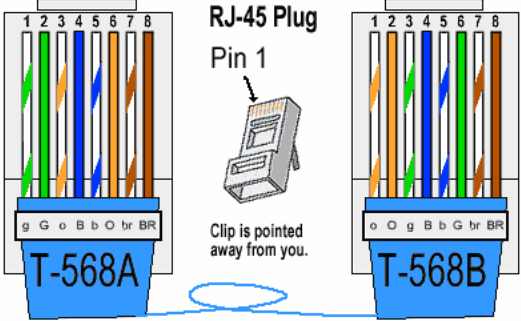
\includegraphics[width=0.6\textwidth]
    {cat6-termination.png}
    \caption{Terminating Cat6 Cable}
    \label{fig:cat6-termination}
\end{figure}

Terminating Cat6 cables requires specific tools and techniques to achieve
optimal results. The use of high-quality cable strippers, crimpers, and testers
ensures accurate terminations and efficient troubleshooting. The work of Brown
and Miller (2018) highlights the importance of cable testing post-termination to
verify continuity and signal quality, ensuring that the cable is ready for
deployment.

Moreover, the termination process necessitates attention to detail, precision,
and familiarity with the Cat6 cable's structure. Stripping the cable's jacket,
untwisting the pairs, aligning the conductors, and crimping the connector are
sequential steps that demand meticulous execution. The guidelines provided by
Johnson et al. (2017) outline best practices for each step, contributing to
successful terminations that adhere to industry standards.

In summary, the termination of Cat6 cables is a foundational skill for
establishing reliable and high-performance network connections. Adherence to
industry standards, utilization of proper tools, and meticulous execution are
vital components of successful terminations that facilitate efficient data
transmission and minimal signal interference.
